\graphicspath{ {pictures} }
\begin{text}

\section{Введение}

	Алгоритм Дейкстры - это алгоритм на графах, который находит кратчайший путь от одной вершины графа к другой. Граф - это структура из точек-вершин, соединенных ребрами-отрезками. Его можно представить как схему дорог или как компьютерную сеть. Ребра - это связи, по ним можно двигаться от одной вершины к другой. Алгоритм Дейкстры работает для графов, у которых нет ребер с отрицательным весом, т.е. таких, при прохождении через которые длина пути как бы уменьшается. Поиск кратчайшего пути в графе является важной задачей в различных областях, таких как:
	\begin{enumerate}
	\item Разработка поведения неигровых персонажей, создание игрового ИИ в геймдеве;
	\item Автоматическая обработка транспортных потоков;
	\item Маршрутизация движения данных в компьютерной сети;
	\item Расчёт движения тока по электрическим цепям.
	\end{enumerate} 
	
\vspace{0.5mm}

	Алгоритм Дейкстры может быть реализован с помощью различных структур данных, таких как куча, очередь с приоритетом или список. Время работы алгоритма зависит от выбранной структуры данных и от различных начальных условий. В данной лабораторной работе будут рассмотрены два алгоритма: на метках и на 3-куче, и в результате будут определены случаи, когда и в какой ситуации будет эффективен один из перечисленных алгоритмов.
\newpage

\section{Постановка задачи}

	Пусть $G = (V, E, W)$ -- ориентированный граф без петель со взвешенными ребрами, где множество вершин $V = \{1,\ldots, n\} $, множество ребер $E \subseteq V\times V, \left| E \right| = m$, и весовая функция $W(u,v)$ каждому ребру $(u, v) \in E$ ставит в соответствие  его вес -- неотрицательное число. Требуется найти кратчайшие пути от заданной вершины $s \in V$ до всех остальных вершин. \\
	
	Если исходный граф не является ориентированным, то для использования описанных алгоритмов следует превратить его в ориентированный, заменив каждое его ребро $(u,v)$ на два ребра $(u,v)$ и $(v,u)$ того же веса. \\
	
	Решением задачи будем считать два массива:
	\begin{itemize}
	\item массив $dist[1..n]$, ($dist[i]$ – кратчайшее расстояние от вершины $s$ до вершины $i$).
	\item массив $all\_path[1..n]$, ($all\_path[i]$ – предпоследняя вершина в построенном кратчайшем пути из вершины $s$ в вершину $i$).
	\end{itemize}
	
	В описываемых алгоритмах $+\infty$ может быть заменено на любое число, превосходящее длину любого кратчайшего пути из вершины $s$ в любую другую вершину графа $G$.\\
	
	В данной лабораторной работе необходимо определить эффективность алгоритмов и их особенности работы.

\newpage
\section{Руководство пользователя}
	Весь проект состоит из двух исполняемых файлов. Первый отвечает за проверку корректности работы обоих алгоритмов, а второй файл производит замеры на различных начальных условиях и записывает время работы в текстовые файлы.\\
	
	При запуске, программа автоматически проводит набор из \textit{семи} тестов, результаты которых записываются в текстовые файлы (1.txt,\ldots,7.txt), находящиеся вместе с исходными файлами в подпапке \textit{Perfomance\_Tests} корневого каталога с приложением.
\newpage

\section{Руководство программиста}
\subsection{Описание структуры программы}

Программа состоит из нескольких модулей и вспомогательных директорий с файлами:
\begin{itemize}
	\item \textbf{boost\_1\_82\_0} -- библиотека \textit{boost} с исходными файлами. Нужна для проверки корректности самостоятельно реализованных алгоритмов Дейкстры. 
	\item \textbf{GTestLib} -- библиотека google test с исходными файлами.
	\item \textbf{include} -- директория с исходными файлами реализации алгоритмов.
		\begin{itemize}
				\item \textbf{d\_heap.hpp} -- исходный файл с шаблонной реалиазации 	структуры данных - \mbox{\textit{D-HEAP}}.
				\item \textbf{generator.hpp} -- исходный файл с шаблонной реализацией генератора целых случайных чисел \textit{(mersenne twister engine)}.
				\item \textbf{graph.hpp, graph.cpp} -- исходные файлы с реализацией основной части программы, а именно: алгоритм Дейкстры с метками и на d-куче, хранение графа, чтение графа из файла и его вывод в текстовые файлы, случайная генерация графа в файл и непосредственно в саму структуру хранения графа.
		\end{itemize}
	\item \textbf{input\_output} -- директория с текстовыми файлами для ввода-вывода графа.
	\item \textbf{Perfomance\_Tests} -- директория с исходными файлами реализацации замеров работы алгоритмов при заданных начальных условиях, текстовыми файлами, в которые записывается время работы в clock'ах. Данные в текстовых файлах расположены в таком порядке: первый столбец - время работы алгоритма Дейкстры на d-куче (в нашем случае 3-куча), второй столбец - время работы алгоритма Дейкстры на метках. 
	\item \textbf{REPORT} -- директория с отчётом о проделанной работе.
	\item \textbf{tests} -- директория с исходными файлами реализации проверки корректности работы обоих алгоритмов Дейкстры, где используется библиотеки \textit{boost} и \textit{google tests}.

\end{itemize}

\newpage
\subsection{Описания модулей и структур данных}
\subsubsection{Описание класса D-HEAP}


\begin{lstlisting}[breaklines=true]
namespace heap {

  template <typename T, size_t dimension>
  class d_Heap {
  public:
    d_Heap(void) = default;
    d_Heap(const std::vector<T>& vector);
    d_Heap(const T* vector, const size_t size);

    ~d_Heap() = default;

    size_t Get_size(void);
    size_t Get_capacity(void);
    bool isEmpty(void);

    size_t first_child(const size_t i);
    size_t last_child(const size_t i);
    size_t father(const size_t i);
    size_t min_child(const size_t i);

    T extract_min(void);
    void push(const T& value);
    T pop(const size_t i);
    void sift_up(size_t i); // Всплытие 
    void sift_down(size_t i); // Погружение
    void make_heap(void);
    void make_heap(const std::vector<T>& vector);
    void make_heap(const T* vector, const size_t size);

    template <typename Tp, size_t d>
    friend std::ostream& operator<<(std::ostream& cout,
      const d_Heap<Tp, d>& heap_);

  private:
    std::vector<T> heap;
  };
\end{lstlisting}
\newpage
\subsubsection{Описание класса generator}

\begin{lstlisting}[breaklines=true]
	namespace gen {
  template <typename T>
  class Random_Generator {
  public:
    Random_Generator();
    Random_Generator(T _min, T _max, size_t seed = std::mt19937::default_seed);

    T generate();
    T generate(T _min, T _max);

  private:
    std::mt19937 gen;
    std::uniform_int_distribution<T> distance;
  };

  template <typename T>
  inline gen::Random_Generator<T>::Random_Generator()
    : distance((T)0, (T)0), gen(std::mt19937::default_seed) {}

  template <typename T>
  inline Random_Generator<T>::Random_Generator(T _min, T _max, size_t seed)
    : distance(_min, _max), gen(seed) {}

  template <typename T>
  inline T Random_Generator<T>::generate() {
    return distance(gen);
  }

  template <typename T>
  inline T Random_Generator<T>::generate(T _min, T _max) {
    distance = std::uniform_int_distribution<T>(_min, _max);
    return distance(gen);
  }

}  // namespace gen
\end{lstlisting}
\newpage
\subsubsection{Описание класса Graph}
\begin{lstlisting}[breaklines=true]
namespace graph {

  struct Edge {
    size_t to, weight;

    bool operator<(const Edge& other) const {
      return this->weight < other.weight;
    }

    bool operator>(const Edge& other) const {
      return this->weight > other.weight;
    }

    bool operator==(const Edge& other) const {
      return this->weight == other.weight;
    }
  };

  using graph_t = std::vector<std::vector<Edge>>;

  class Graph {
  public:
    Graph() = default;
    ~Graph() = default;

    void init_from_file(const char* path);

    void generate_to_file(const char* path, const size_t num_vertices,
      const size_t num_edges, const size_t min_weight,
      const size_t max_weight);
    void generate_to_graph(const size_t num_vertices, const size_t num_edges,
      const size_t min_weight, const size_t max_weight);
    void write_to_file(const char* path,
      const size_t finish_vertex = RESERVE_SIZE_MAX);

    std::vector<size_t>& Dijkstra_Mark();
    std::vector<size_t>& Dijkstra_3Heap();

    std::vector<size_t>& Get_path(const size_t finish_vertex);
    size_t Get_vertexCount() const;
    size_t Get_edgeCount() const;
    size_t Get_startVertex() const;
    void Set_startVertex(const size_t node);
    void clear_paths_and_dist();

    std::vector<Edge>& operator[](const size_t index);
    const std::vector<Edge>& operator[](const size_t index) const;

  private:
    graph_t graph;
    std::vector<size_t> all_paths;
    std::vector<size_t> path;
    std::vector<size_t> dist;
    size_t vertexCount = (size_t)0, edgeCount = (size_t)0;
    size_t start_vertex;
  };

}  // namespace graph
\end{lstlisting}
\newpage

\subsubsection{Описание модуля Test (Проверка на корректность)}

\begin{lstlisting}[breaklines=true]
const char* input_file_path = "..\\..\\input_output\\input.txt";
const char* input_file_path_2 = "..\\..\\input_output\\input_2.txt";
const char* input_file_path_3 = "..\\..\\input_output\\input_3.txt";
const char* output_file_path = "..\\..\\input_output\\output.txt";

using boost_Graph =
boost::adjacency_list<boost::listS, boost::vecS, boost::directedS,
  boost::no_property,
  boost::property<boost::edge_weight_t, size_t> >;
using Vertex = boost::graph_traits<boost_Graph>::vertex_descriptor;
using Edge = std::pair<size_t, size_t>;

TEST(TEST_NATIVE_DIJKSTRA, The_First_TEST){...}
TEST(TEST_NATIVE_DIJKSTRA, The_Second_TEST){...}
TEST(TEST_NATIVE_DIJKSTRA, BOOST_ONE_TEST){...}
TEST(TEST_NATIVE_DIJKSTRA, BOOST_ONE_RANDOM_GENERATE_TO_GRAPH_TEST){...}
TEST(TEST_NATIVE_DIJKSTRA, BOOST_LOT_RANDOM_TESTS){...}
\end{lstlisting}
\newpage

\subsubsection{Описание модуля Perfomance Tests (Замеры времени)}
\begin{lstlisting}[breaklines=true]
using time_type = std::chrono::steady_clock::time_point;
using time_n = std::chrono::nanoseconds;
using time_ml = std::chrono::milliseconds;
using time_mc = std::chrono::microseconds;
using time_s = std::chrono::seconds;

namespace perf {
  const char* path1 = "..\\..\\Perfomance_Tests\\1.txt";
  const char* path2 = "..\\..\\Perfomance_Tests\\2.txt";
  const char* path3 = "..\\..\\Perfomance_Tests\\3.txt";
  const char* path4 = "..\\..\\Perfomance_Tests\\4.txt";
  const char* path5 = "..\\..\\Perfomance_Tests\\5.txt";
  const char* path6 = "..\\..\\Perfomance_Tests\\6.txt";
  const char* path7 = "..\\..\\Perfomance_Tests\\7.txt";

  void test_measurement_1();
  void test_measurement_2();
  void test_measurement_3();
  void test_measurement_4();
  void test_measurement_5();
  void test_measurement_6();
  void test_measurement_7();
}  // namespace perf
\end{lstlisting}
\newpage

\subsection{Алгоритмическая сложность алгоритмов Дейкстры}
\subsubsection{Алгоритм Дейкстры на метках}

Повторить $V$ раз:
\begin{itemize}
	\item Из всех вершин, расстояния до которых ещё не являются окончательными, выбрать ближайшую и пометить расстояние до неё как окончательное.
	\item Затем посмотреть рёбра из этой вершины и попробовать улучшить расстояния до вершин-соседей.
\end{itemize}

В алгоритме Дейкстры требуется $V$ раз определять ближайшую вершину и не более $2E$ раз (в сумме по всем вершинам) производить релаксации (уменьшее расстояния до вершины).\\

Если мы используем только массив расстояний, то:
\begin{itemize}
	\item Сложность определения ближайшей вершины равна $O(V)$.
	\item Сложность одной релаксации равна $O(1)$.
\end{itemize}

Таким образом, общая сложность алгоритма Дейкстры на метках составляет \textbf{$O(V^2 + E)$}.\\

\subsubsection{Алгоритм Дейкстры на d-куче}
\textit{В данной лабораторной работе подразумевается использование только 3-кучи.}

Алгоритмическая сложность основных методов d-кучи:
\begin{enumerate}
	\item[--] Добавление: $O(\log_d(n))$;
	\item[--] Удаление: $O(d * \log_d(n))$;
	\item[--] Погружение: $O(d * \log_d(n))$;
	\item[--] Всплытие: $O(\log_d(n))$;
	\item[--] Взятие минимума: $O(\log_d(n))$.
\end{enumerate}

Если мы храним необработанные вершины в d-куче, то:
\begin{itemize}
	\item Сложность определения ближайшей вершины равна $O(\log(V))$.
	\item Сложность одной релаксации также равна $O(\log(V))$.
\end{itemize}

Таким образом, общая сложность алгоритма составляет $O((V + E)\log(V))$.\\

Первый вариант на метках более эффективен для плотных графов,\\
второй вариант на d-куче более эффективен для разреженных графов.
\newpage

\section{Заключение}
\textbf{\textit{Все замеры проводились на данной рабочей машине:}}
\begin{enumerate}
	\item[--] \textbf{ОС}: Windows 10 Pro x64 (2009 build 19044)
	\item[--] \textbf{Процессор}: Intel(R) Xeon(R) CPU E3-1270 v3 @ 3.50GHz
	\item[--] \textbf{ОЗУ}: 16 ГБ DDR3
\end{enumerate}

Далее представлены семь графиков с замерами работы алгоритмов Дейкстры на метках и на d-куче.\\

% ТЕСТЫ -----------------------------------------------------------------------------
\begin{center}
\textbf{\textit{Тест №1}}
\textbf{Начальные условия:}

\begin{enumerate}
	\item[--] Количество вершин -- n: $1,...,10^4 + 1$, \textbf{шаг} -- $100$
	\item[--] Левая граница веса ребра: $1$
	\item[--] Правая граница веса ребра: $10^6$
	\item[--] Количество рёбер -- m: $\dfrac{n^2}{10}$ 
\end{enumerate}

\end{center}
\begin{figure}[h]
  \centering
  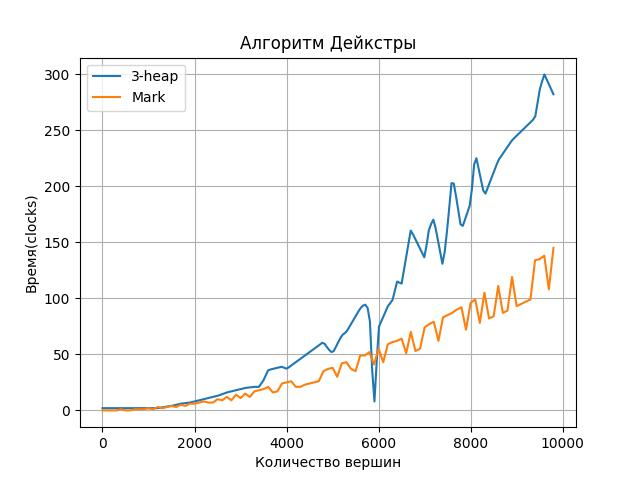
\includegraphics[width=0.8\textwidth]{pictures/1.jpeg}
  \caption{Тест №1}
  \label{fig:pict_1}
\end{figure}

	На данном примере явно видно, что алгоритм на d-куче медленнее, так как у нас большое количество рёбер. И как говорилось ранее, алгоритм на d-куче будет эффективен только на разреженном графе. Поэтому на данных начальных условиях по всем параметрам выигрывает алгоритм на метках.\\
	
\begin{center}
\textbf{\textit{Тест №2}}
\textbf{Начальные условия:}

\begin{enumerate}
	\item[--] Количество вершин -- n: $1,...,10^4 + 1$, \textbf{шаг} -- $100$
	\item[--] Левая граница веса ребра: $1$
	\item[--] Правая граница веса ребра: $10^6$
	\item[--] Количество рёбер -- m: $n^2$ 
\end{enumerate}

\end{center}
\begin{figure}[h]
  \centering
  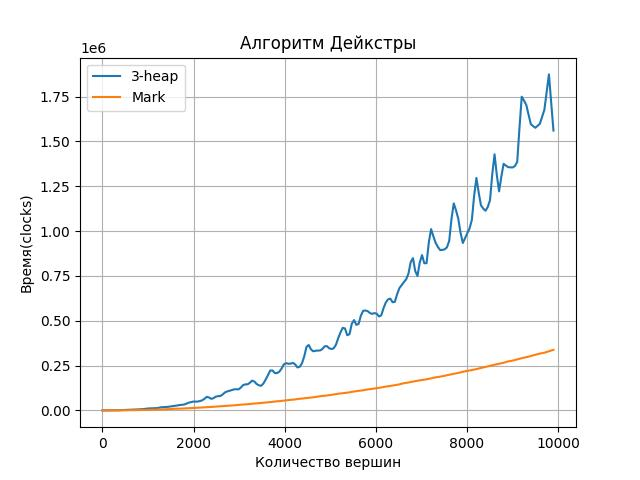
\includegraphics[width=0.8\textwidth]{pictures/2.jpeg}
  \caption{Тест №2}
  \label{fig:pict_2}
\end{figure}

На данном примере граф является и вовсе полным, поэтому здесь выигрывает алгоритм на метках, так же как и в первом тесте.\\
\newpage
\begin{center}
\textbf{\textit{Тест №3}}
\textbf{Начальные условия:}

\begin{enumerate}
	\item[--] Количество вершин -- n: $101,...,10^4 + 1$, \textbf{шаг} -- $100$
	\item[--] Левая граница веса ребра: $1$
	\item[--] Правая граница веса ребра: $10^6$
	\item[--] Количество рёбер -- m: $100*n$ 
\end{enumerate}

\end{center}
\begin{figure}[h]
  \centering
  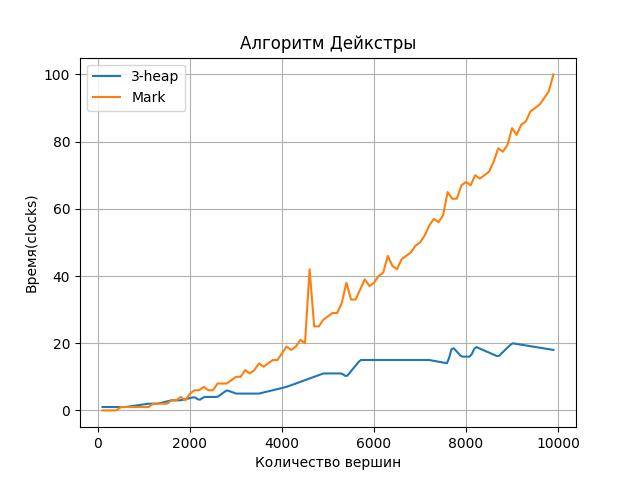
\includegraphics[width=0.8\textwidth]{pictures/3.jpeg}
  \caption{Тест №3}
  \label{fig:pict_3}
\end{figure}

На данном примере графики ведут уже себя по-другому. Так как количество рёбер $m = 100*n$, то чем больше количество вершин - тем больее эффективен будет алгоритм на d-куче. Только на начальных итерациях, когда количество вершин меньше $2000$ граф является плотным, поэтому скорость работы обоих алгоритмов практически одинаковая.\\
\newpage

\begin{center}
\textbf{\textit{Тест №4}}
\textbf{Начальные условия:}

\begin{enumerate}
	\item[--] Количество вершин -- n: $101,...,10^4 + 1$, \textbf{шаг} -- $100$
	\item[--] Левая граница веса ребра: $1$
	\item[--] Правая граница веса ребра: $10^6$
	\item[--] Количество рёбер -- m: $1000*n$ 
\end{enumerate}

\end{center}
\begin{figure}[h]
  \centering
  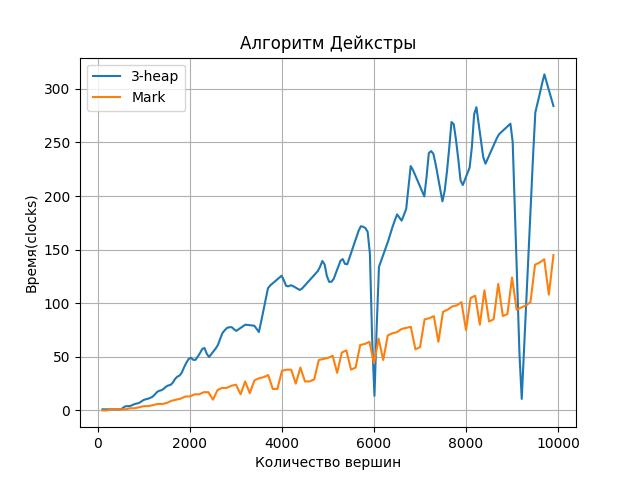
\includegraphics[width=0.8\textwidth]{pictures/4.jpeg}
  \caption{Тест №4}
  \label{fig:pict_4}
\end{figure}

По сравнению с предыдущим тестом, количество рёбер увеличилось на порядок. Поэтому алгоритм на d-куче вновь стал проигрывать алгоритму на метках, так как граф стал опять плотным.\\
\newpage

\begin{center}
\textbf{\textit{Тест №5}}
\textbf{Начальные условия:}

\begin{enumerate}
	\item[--] Количество вершин -- n: $10^4 + 1$
	\item[--] Левая граница веса ребра: $1$
	\item[--] Правая граница веса ребра: $10^6$
	\item[--] Количество рёбер -- m: $0,...,10^7$, \textbf{шаг} -- $10^5$
\end{enumerate}

\end{center}
\begin{figure}[h]
  \centering
  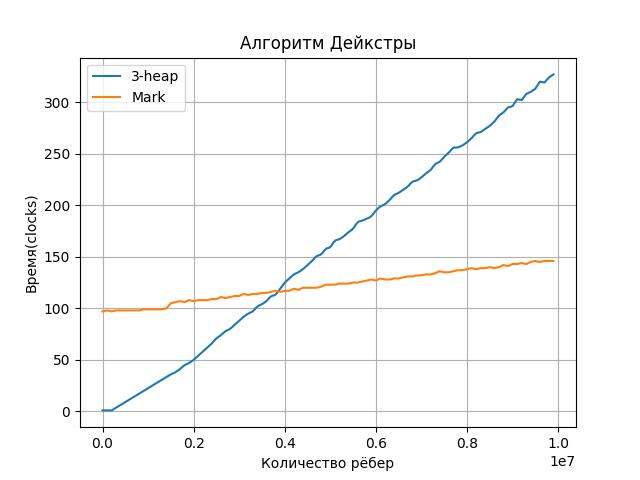
\includegraphics[width=0.8\textwidth]{pictures/5.jpeg}
  \caption{Тест №5}
  \label{fig:pict_5}
\end{figure}

Данный пример является самым показательным и наглядным. Видно, что переходя граничную точку по количеству рёбер, алгоритм на d-куче будет работать медленнее, потому что граф становится плотным.\\
\newpage

\begin{center}
\textbf{\textit{Тест №6}}
\textbf{Начальные условия:}

\begin{enumerate}
	\item[--] Количество вершин -- n: $10^4 + 1$
	\item[--] Левая граница веса ребра: $1$
	\item[--] Правая граница веса ребра: $1,...,200$, \textbf{шаг} -- $1$
	\item[--] Количество рёбер -- m: $n^2$
\end{enumerate}

\end{center}
\begin{figure}[h]
  \centering
  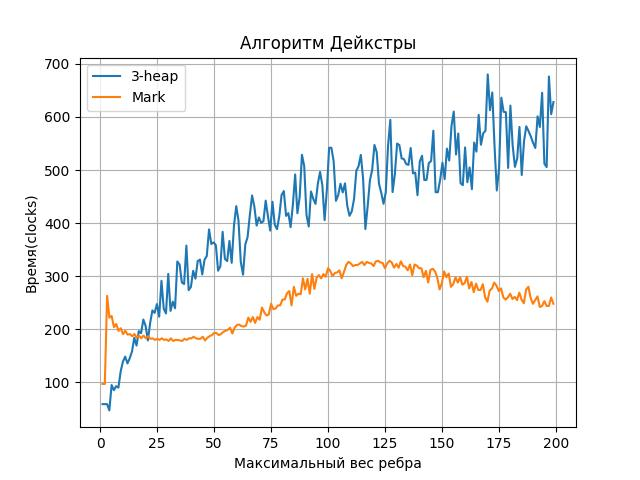
\includegraphics[width=0.8\textwidth]{pictures/6.jpeg}
  \caption{Тест №6}
  \label{fig:pict_6}
\end{figure}

Так как количество рёбер $n^2$, можно определить, что граф является полным. Но судя по графку на маленьких значениях правой границы веса ребра алгоритм на d-куче всё-же выигрывает. Это объясняется тем, что при увелечинии максимального веса ребра, в методе d-кучи - \guillemotleft Всплытие \guillemotright ,может происходить больше итераций, чем когда разброс значений маленький. То есть вся разница в константе, которая не пишется при определении алгоритмической сложности алгоритма.\\
\newpage

\begin{center}
\textbf{\textit{Тест №7}}
\textbf{Начальные условия:}

\begin{enumerate}
	\item[--] Количество вершин -- n: $10^4 + 1$
	\item[--] Левая граница веса ребра: $1$
	\item[--] Правая граница веса ребра: $1,...,200$, \textbf{шаг} -- $1$
	\item[--] Количество рёбер -- m: $1000 * n$
\end{enumerate}

\end{center}
\begin{figure}[h]
  \centering
  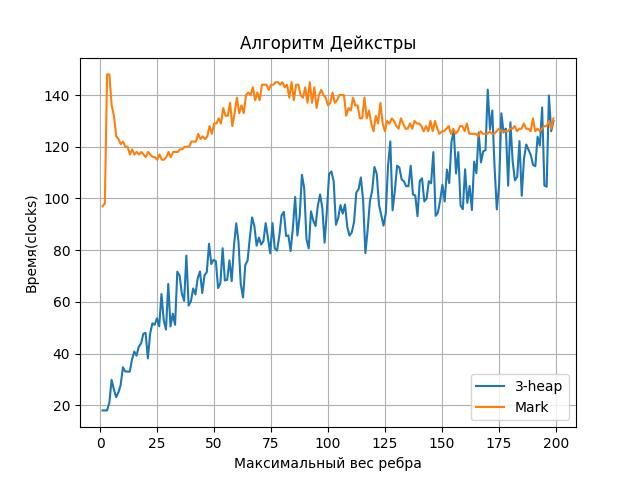
\includegraphics[width=0.8\textwidth]{pictures/7.jpeg}
  \caption{Тест №7}
  \label{fig:pict_7}
\end{figure}

На данном примере похожая ситуация, как и в предыдущем случае. Разница лишь в том, что граф не настолько плотный, чем в тесте №6. Но при увеличении максимального веса ребра алгоритм на d-куче становится медленнее. Поэтому уже при максимальном весе около $200$ время работы алгоритмов практически одинаковое. Если ещё увеличивать максимальную границу веса ребра, то выигрывать конечно же алгоритм на метках.\\

\textbf{Вывод}:\\
В результате проделанной работы все поставленные задачи выполнены. Оба алгоритма эффективны при определённых начальных условиях. Поэтому, в зависимости от требований, следует выбирать тот алгоритм, который будет иметь преимущество именно в этой ситуации.
\newpage

\section{Литература}

\begin{enumerate}
	\item Мой GitHub. \url{https://github.com/Sturmannn/Lab_Dijkstra_algorithm}
	\item Википедия. \href{https://ru.wikipedia.org/wiki/%D0%90%D0%BB%D0%B3%D0%BE%D1%80%D0%B8%D1%82%D0%BC_%D0%94%D0%B5%D0%B9%D0%BA%D1%81%D1%82%D1%80%D1%8B}{https://ru.wikipedia.org/wiki/Алгоритм\_Дейкстры}
	\item YouTube. \href{https://www.youtube.com/watch?v=J-7MzbEtTR0&t=2s}{Алгоритм Дейкстры: два варианта реализации}
	\item Университет ИТМО. \href{https://neerc.ifmo.ru/wiki/index.php?title=%D0%90%D0%BB%D0%B3%D0%BE%D1%80%D0%B8%D1%82%D0%BC_%D0%94%D0%B5%D0%B9%D0%BA%D1%81%D1%82%D1%80%D1%8B}{Алгоритм Дейкстры -- Викиконспекты}
\end{enumerate}

\end{text}
